\documentclass[times, utf8, zavrsni]{fer}
\usepackage{booktabs}
\usepackage{mathtools}
\usepackage{graphicx}
\usepackage{hyperref}
\usepackage{algorithm}
\usepackage[noend]{algpseudocode}
\usepackage{amsmath}
\DeclareUnicodeCharacter{2009}{ }
% \renewcommand{\algorithmcfname}{Algoritam}%
\floatname{algorithm}{Algoritam}

\usepackage{listings}
\usepackage{color}

\definecolor{dkgreen}{rgb}{0,0.6,0}
\definecolor{gray}{rgb}{0.5,0.5,0.5}
\definecolor{mauve}{rgb}{0.58,0,0.82}

\lstset{frame=tb,
  language=C++,
  aboveskip=3mm,
  belowskip=3mm,
  showstringspaces=false,
  columns=flexible,
  basicstyle={\small\ttfamily},
  numbers=none,
  numberstyle=\tiny\color{gray},
  keywordstyle=\color{blue},
  commentstyle=\color{dkgreen},
  stringstyle=\color{mauve},
  breaklines=true,
  breakatwhitespace=true,
  tabsize=3
}

\begin{document}

% TODO: Navedite broj rada.
\thesisnumber{000}

% TODO: Navedite naslov rada.
\title{Landau-Vishkin-Nussinov algoritam za poravnanje dva niza}

% TODO: Navedite vaše ime i prezime.
\author{Donik Vršnak}

\maketitle

% Ispis stranice s napomenom o umetanju izvornika rada. Uklonite naredbu \izvornik ako želite izbaciti tu stranicu.
\izvornik

% Dodavanje zahvale ili prazne stranice. Ako ne želite dodati zahvalu, naredbu ostavite radi prazne stranice.
\zahvala{}

\tableofcontents

\chapter{Uvod}
Problem pronalaženja homolognih poklapanja unutar dva niza je problem koji je značajan za mnoga područja moderne znanosti, a pogotovo je važan u području bioinformatike. Zbog brzog razvoja različitih metoda sekvenciranja genoma, koje postaju sve jeftinije i pristupačnije, u bioinformatici se javila potreba za razvojem algoritama koji mogu efikasno rješavati problem pronalaženja poravnanja homolognih preklapanja unutar genoma. Sekvenciranjem genoma dobivamo sekvence koje je moguće jednostavno prikazati u računalu, jer se svaka aminokiselina može preslikati u jedan znak. Drugim riječima, jedno očitanje molekule DNK se može preslikati u niz znakova. Time se problem pronalaženja sličnih dijelova sekvenci dobivenih sekvenciranjem DNK pretvara u problem pronalaženja preklapanja unutar dva niza znakova. Također, vidljivo je da se ovakvi algoritmi mogu primjenjivati na bilo koja dva niza znakova, no u ovom radu fokusirat ćemo se na njihovu primjenu u bioinformatici i preklapanju sekvenci DNK.

Iako se na prvi pogled taj problem može činiti jednostavnim, do problema dolazimo kada u obzir uzmemo moguće duljine sekvenci koje mogu imati od nekoliko desetaka proteinskih baza, pa i do čak nekoliko stotina tisuća proteinskih baza, a da ukupni broj baza u svim sekvencama može biti i do nekoliko desetaka milijardi. Ako bi problem probali riješiti nekim jednostavnim algoritmom koji bi, ako uspoređujemo dvije sekvence od kojih jedna ima duljinu \textit{m}, a druga duljinu \textit{n}, njegova složenost bila bi \textit{O}(\textit{nm}), vidljivo je da bi vrijeme potrebno za rješavanje bilo preveliko. Zbog toga dolazimo do potrebe za efikasnijim algoritmima poravnanja, koje možemo podijeliti na heurističke i analitičke. Heuristički algoritmi se baziraju na procjeni poravnanja korištenjem različitih heurističkih funkcija te su samim time nešto neprecizniji od analitičkih, ali tu nepreciznost nadoknađuju u brzini pronalaženja rješenja. S druge strane, analitički algoritmi uvode neka ograničenja na rješenja, te si time smanjuju ukupni prostor rješenja koje moraju pretražiti. Algoritam Landau-Vishkin-Nussinov spada u skupinu analitičkih algoritama te će dalje u radu biti razmatrani samo analitički algoritmi.

U suštini, problem traženja poravnanja između dva niza svodi se na traženje najmanjeg broja razlika između ta dva niza, pronalaska mjesta na kojima se te razlike pojavljuju te njihove vrste. Najčešća podjela razlika je na tri vrste:
\begin{enumerate}
\item brisanje znaka iz niza
\item umetanje znaka u niz
\item izmjena jednog znaka drugim znakom
\end{enumerate}
Drugi naziv za broj razlika između dva niza je Levenshteinova udaljenost (eng. edit distance), koju ćemo dalje u radu, radi jednostavnosti, nazivati samo udaljenost. Udaljenost dva niza možemo promatrati i kao broj transformacija nad pojedinim znakovima koje je potrebno napraviti da bi se prvi niz pretvorio u drugi niz. Također, radi jednostavnosti uvest ćemo nazive za dva niza koja uspoređujemo, tako da ćemo kraći niz prozvati uzorak, a duži tekst. Na primjer, najmanja udaljenost između uzorka "Hello" i teksta "World!" je 5 jer sve znakove osim znaka \textit{l} moramo promijeniti kako bi iz niza "Hello" dobili niz "World!".

\section{Cilj rada}
Cilj ovog rada bio je implementirati algoritam poravnanja dva niza koji su predložili Gad M. Landau, Uzi Vishkin i Ruth Nussinov \citep{Landau1986}. Također nakon implementacije, performanse implementacije algoritma smo uspoređivali s implementacijom Myers-ovog bit-vektor algoritma \citep{Myers1999} koja se koristi u alatu za određivanje poravnanja parova nizova edlib \citep{edlib}. Kako je Myersov algoritam sporiji u slučajevima kada se radi o poravnanju kratkih nizova, dodatni cilj rada bio je integrirati implementirani algoritam u alat edlib, te odrediti jednostavnu heurističku funkciju koja će odrediti koju implementaciju je potrebno koristiti, u ovisnosti o duljinama ulaznih nizova.

\chapter{Pregled pojmova}
\section{Metode poravnavanja}
Metode poravnanja dijele se u tri glavne skupine: globalne, lokalne i polu-globalne. Ove metode razlikuju se u načinu na koji se penaliziraju transformacija unutar teksta. Kod lokalnog poravnanja tražimo slična područja unutar dva niza, odnosno uspoređujemo sličnost nizova s obzirom na podnizove određenih duljina. Najpoznatiji takav algoritam je Smith-Watermanov algoritam \citep{Smith1981}, koji koristi dinamičko programiranje za pronalaženje optimalnog lokalnog poravnanja. S druge strane, u globalnim metodama provodi se uspoređivanje nizova na temelju pojedinačnih znakova, odnosno određivanju udaljenosti nizova. Kod čistih globalnih algoritama, uzorka svaka transformacija se penalizira, obično s cijenom 1, kao što je prije navedeno. No, kod polu-globalnih metoda, dopuštamo da se transformacije na početku i/ili na kraju nizova ne penaliziraju. Ako cijenu transformacija na početku i na kraju niza zanemarujemo, tada globalni algoritam prelazi u infiksni, a ako zanemarujemo cijenu transformacija samo na kraju niza tada algoritam prelazi u prefiksni. Iz ovoga je vidljivo da su globalni algoritmi primjenjivi na nizove slične duljine, dok su polu-globalni bolji u slučajevima kada je tekst mnogo duži od uzorka. U ovome radu fokusirat ćemo se samo na globalne i polu-globalne algoritme. Osnovni algoritam za globalno poravnanje je Needleman-Wunschov algoritam \citep{Needleman1970}, koji dinamičkim programiranjem pronalazi poravnanje. Problem ovog algoritma je njegova vremenska složenost, koja iznosi \textit{O}(\textit{nm}), gdje je \textit{m} duljina uzorka, a \textit{n} duljina teksta. Zbog toga je došlo do razvoja mnogih drugih algoritama koji pokušavaju smanjiti vremensku složenost, kao što su Ukkonen-ov algoritam \citep{Ukkonen1985}, koji složenost smanjuje pametnim ograničavanjem prostora pretraživanja te Hirschebergov algoritam \citep{Hirschberg1975}, koji prostornu složenost smanjuje na linearnu u zamjenu za nešto duže vrijeme izvođenja.

\section{Poravnanje}
\begin{sloppypar}
Poravnanje dva niza, uzorka $R$ i teksta $B$, je postupak u kojem se u tekstu pokušavaju pronaći područja koja su slična uzorku. Sličnost uzorka i područja unutar teksta definira se pomoću njihove udaljenosti, odnosno broja transformacija nad pojedinim znakovima koje se moraju primijeniti na uzorak kako bi se on u potpunosti podudarao s odabranim područjem u tekstu. Pretpostavimo da je uzorak \(R = r_{0}r_{1}...r_{i-1}r_{i}r_{i+1}...r_{m-1}r_{m}\). Dopuštene transformacije na uzorku su:
\begin{enumerate}
\item brisanje znaka na poziciji \textit{i} iz niza. Uzorak tada postaje \(R = r_{0}r_{1}...r_{i-1}r_{i+1}...r_{m-1}r_{m}\).
\item umetanje znaka \textit{z} u niz na poziciju \textit{i}. Novi uzorak je \(R = r_{0}r_{1}...r_{i-1}r_{i}zr_{i+1}...r_{m-1}r_{m}\).
\item zamjena znaka na poziciji \textit{i} znakom \textit{z}, čime uzorak postaje \(R = r_{0}r_{1}...r_{i-1}zr_{i+1}...r_{m-1}r_{m}\).
\end{enumerate}
\end{sloppypar}
Prilikom određivanja udaljenosti, svaka od ovih transformacija može se penalizirati te se tada udaljenost uzorka od teksta definira kao zbroj svih vrijednosti penala transformacija (cijena transformacija) potrebnih da se uzorak transformira u tekst. Zbog jednostavnosti, ako nije drugačije navedeno, vrijednosti penala za svaku transformaciju bit će jednake te će iznositi 1, odnosno $C_{CH} = C_{DE} = C_{IN} = 1$, gdje $C_{CH}$ predstavlja cijenu zamjene znaka, $C_{DE}$ cijenu brisanja znaka, a $C_{IN}$ cijenu umetanja znaka.

\section{CIGAR format}\label{sec:cigar}
Za prikaz rezultata poravnanja koristi se format CIGAR, koji je jedan od standardnih formata korištenih u bioinformatici. On se sastoji od oznake početne pozicije u tekstu od koje uspoređujemo uzorak i tekst, te od niza znakova koji predstavljaju broj znakova te transformacija koje se odnose na te znakove. Postoje dvije vrste CIGAR formata, standardni i prošireni. U standardnom formatu zamjena znaka i poklapanje znakova unutar uzorka i teksta se označavaju znakom "M", umetanje znaka u tekst označava se znakom "I", a brisanje znaka iz teksta označava se znakom "D". Za razliku od toga, prošireni CIGAR format razlikuje zamjenu znakova, koja se označava znakom "X", i poklapanje znakova, koje se označava znakom "M". Na primjer, za uzorak $R = ACTAGAATGGCT$ i tekst $B = CCATACTGAACTGACTAAC$, rezultat infiks poravnanja prikazan u standardnom CIGAR formatu bio bi:
\begin{flushleft}
$POS: 5$
\linebreak $CIGAR: 3M1I3M1D5M $,
\linebreak dok bi u proširenom CIGAR formatu to bilo:
\linebreak $POS: 5$
\linebreak $CIGAR: 3{=}1I3{=}1D2{=}1X2{=}$ .
\end{flushleft}

\section{Edlib}
Edlib \citep{edlib} je c/c++ implementacija Myersovog bit vektor algoritma \citep{Myers1999} za pronalaženje globalnog poravnanja između dva niza. Uz Myersov algoritam, edlib još koristi i Hirschebergov \citep{Hirschberg1975} i Ukkonenov \citep{Ukkonen1985} algoritam. Iako mu je složenost i dalje kvadratna, edlib je jako brz za dugačke slične nizove, jer se za njih dobiva najveće ubrzanje. No, edlib, zbog algoritama koje koristi, ima problem s kratkim nizovima, do otprilike 500 proteinskih baza, te je zato bilo potrebno ugraditi novi algoritam koji će moći brže rješavati problem za kratke nizove. Edlib podržava traženje globalnog, prefiksnog i infiksnog poravnanja dva niza, te omogućava prikaz rezultata poravnanja u formatu CIGAR.

\chapter{Algoritam Landau-Vishkin-Nussinov}
\section{Definicija problema}
Generalno, problem koji je potrebno riješiti je efikasno odrediti poravnanja između dva niza \(R = r_{0}r_{1}{\dots}r_{m-1}r_{m}\) i \(B = b_{0}b_{1}{\dots}b_{n-1}b_{n}\), gdje u našem slučaju, abecede sadrže samo znakove $A,C,T,G$. Ovaj problem možemo podijeliti na dva potproblema, a to su pronalaženje najmanje udaljenosti između nizova $R$ i $B$, te pronalaženja točnih transformacija nad nizovima za koji se taj minimum postiže. Taj problem još se naziva problem traženja optimalnog puta za neko poravnanje. 

Razlikujemo tri vrste poravnanja, globalno, prefiksno i infiksno. Globalno poravnanje je poravnanje kod kojega se svaka razlika između dva niza ubraja u konačnu udaljenost. Za razliku od toga, kod prefiksnog i infiksnog algoritma, prilikom izračunavanja udaljenosti zanemarujemo razlike uzorka $R$ i teksta $B$ na početku ili na kraju teksta. Tako, kod prefiksnog algoritma u rezultat ulaze samo cijene transformacija koje dobivamo dok nismo došli do kraja uzorka $R$. Infiksno poravnanje slično je prefiksnom samo što dopuštamo zanemrivanje cijena i s početka teksta $B$, drugim riječima, dopuštamo da poravnanje uzorka ne počinje od prve pozicije teksta $B$. Demonstrirajmo to na primjeru uzorka $R = AGCGCTTGCTGC$ i teksta $B = AGTCGCCGCTGCTGC$. Rezultati ove tri vrste poravananja dani su na slijedećoj slici.

\subsection{Pronalaženje minimalne udaljenosti}
\label{subsec:osnovniAlgoritam}
Pretpostavimo, bez smanjenja općenitosti, da se je $m{\leq}n$. Tada niz $R$ možemo prozvati uzorkom, a niz $B$ tekstom. Nizovi $R$ i $B$ mogu se razlikovati na $0{\leq}i{\leq}m$ mjesta, a te promjene (mutacije) mogu biti brisanje, umetanje i izmjena znaka. Svaku od tih razlika možemo penalizirati s cijenom 1, te se tada naš problem pretvara u traženje minimalnog broja transformacija koje uzorak $R$ pretvaraju u tekst $B$. Ovako definiran problem odgovara globalnom poravnanju nizova. Prefiksno poravnanje možemo lagano dobiti iz globalnog tako da zbrajanje cijena prekinemo kada dođemo do kraja uzorka, a infiksno poravnanje odgovara prefiksnom, s mogućnošću da preklapanje uzorka i teksta počinjemo od proizvoljne pozicije unutar teksta.
Matrica $D$ je matrica $m{\times}n$ koja sadrži vrijednosti udaljenosti uzorka i teksta, dok se uz $y$ os ($i=1{\dots}m$) matrice proteže uzorak $R$, a uz $x$ os ($j=1{\dots}n$) tekst $B$. Drugim riječima, $D_{i,j}$ predstavlja udaljenost podnizova $r_{1}{\dots}r_{i}$ i $b_{1}{\dots}r_{j}$. Također, vidljivo je da povećanje vrijednosti $i{\rightarrow}i+1$ odgovara pomicanju po uzorku, povećanje vrijednosti $j{\rightarrow}j+1$ pomicanju po tekstu, dok je istovremeno pomicanje po uzorku i tekstu predstavljeno kao istovremeno povećanje vrijednosti $i$ i $j$ ($i{\rightarrow}i+1, j{\rightarrow}j+1$). U biološkom smislu, pomicanje samo po uzorku ($i{\rightarrow}i+1$) odgovara brisanju znaka iz uzorka, pomicanje samo po tekstu ($j{\rightarrow}j+1$)odgovara umetanju znaka u uzorak, a pomicanje i po uzorku i po tekstu ($i{\rightarrow}i+1, j{\rightarrow}j+1$) odgovara ili poklapanju u slučaju da je $r_{i}=b_{j}$ ili izmjeni ako $r_{i} \neq b_{j}$.

Vidljivo je da je kretanje po nekoj dijagonali $d = j-i$ poželjnije nego kretanje po retku ili stupcu, jer svako takvo kretanje sigurno povećava broj transformacija, dok se kretanjem po dijagonali taj broj, u slučaju poklapanja, neće povećavati. Matrica koja nastaje ovakvim kretanjem kroz uzorak $R = ACTAGAATGGCT$ i tekst $B = CCATACTGAACTGACTAAC$ prikazana je u tablici \ref{tab:matricaDij}. Ova matrica može se jednostavno izračunati pomoću algoritma (\ref{alg:osnovni}) koji je dan u nastavku.

\begin{algorithm}
\caption{Osnovni algoritam za izračunavanje udaljenosti dva niza}\label{alg:osnovni}
\begin{algorithmic}
\State $D_{0,0} \gets 0$
\State $C_{CH}\gets 1$ 
\State $C_{DE} \gets 1$
\State $C_{IN} \gets 1$
\ForAll{$i, 1\leq i\leq m$} \State $D_{i,0} \gets i$ \EndFor
\ForAll{$j, 1\leq j\leq n$} \State $D_{j,0} \gets j$ \EndFor
\linebreak
\For{$i \gets 1$ to $m$}
    \For{$j \gets 1$ to $n$}
        \State $D_{i,j} \gets min(D_{i-1,j}+C_{DE}, D_{i.j-1}+C_{IN}, D_{i-1,j-1} $ if $r_{i}=b_{j} $ or $ D_{i-1,j-1}+C_{CH})$
    \EndFor
\EndFor
\end{algorithmic}
\end{algorithm}

\begin{table}[]
\begin{tabular}{|ll|llllllllllllllll|}
\hline
                         &   & 0                               & 1                               & 2                               & 3                               & 4                               & 5                               & 6                               & 7                               & 8                               & 9                               & 10                              & 11                              & 12                              & 13                      & 14                      & 15 \\ \cline{3-18} 
                         &   & \multicolumn{1}{l|}{}           & A                               & G                               & T                               & C                               & G                               & C                               & C                               & G                               & C                               & T                               & G                               & C                               & T                       & G                       & C  \\ \hline
\multicolumn{1}{|l|}{0}  &   & \multicolumn{1}{l|}{\textbf{0}} & \multicolumn{1}{l|}{1}          & \multicolumn{1}{l|}{2}          & \multicolumn{1}{l|}{3}          & \multicolumn{1}{l|}{4}          & \multicolumn{1}{l|}{5}          & \multicolumn{1}{l|}{6}          & \multicolumn{1}{l|}{7}          & \multicolumn{1}{l|}{8}          & \multicolumn{1}{l|}{9}          & \multicolumn{1}{l|}{10}         & \multicolumn{1}{l|}{11}         & \multicolumn{1}{l|}{12}         & \multicolumn{1}{l|}{13} & \multicolumn{1}{l|}{14} & 15 \\ \cline{2-18} 
\multicolumn{1}{|l|}{1}  & A & \multicolumn{1}{l|}{1}          & \multicolumn{1}{l|}{\textbf{0}} & \multicolumn{1}{l|}{1}          & \multicolumn{1}{l|}{2}          & \multicolumn{1}{l|}{3}          & \multicolumn{1}{l|}{4}          & \multicolumn{1}{l|}{5}          & \multicolumn{1}{l|}{6}          & \multicolumn{1}{l|}{7}          & \multicolumn{1}{l|}{8}          & \multicolumn{1}{l|}{9}          & \multicolumn{1}{l|}{10}         & \multicolumn{1}{l|}{11}         & \multicolumn{1}{l|}{12} & \multicolumn{1}{l|}{13} & 14 \\ \cline{3-18} 
\multicolumn{1}{|l|}{2}  & G & \multicolumn{1}{l|}{2}          & \multicolumn{1}{l|}{1}          & \multicolumn{1}{l|}{\textbf{0}} & \multicolumn{1}{l|}{1}          & \multicolumn{1}{l|}{2}          & \multicolumn{1}{l|}{3}          & \multicolumn{1}{l|}{4}          & \multicolumn{1}{l|}{5}          & \multicolumn{1}{l|}{6}          & \multicolumn{1}{l|}{7}          & \multicolumn{1}{l|}{8}          & \multicolumn{1}{l|}{9}          & \multicolumn{1}{l|}{10}         & \multicolumn{1}{l|}{11} & \multicolumn{1}{l|}{12} & 13 \\ \cline{3-18} 
\multicolumn{1}{|l|}{3}  & C & \multicolumn{1}{l|}{3}          & \multicolumn{1}{l|}{2}          & \multicolumn{1}{l|}{1}          & \multicolumn{1}{l|}{\textbf{1}} & \multicolumn{1}{l|}{\textbf{1}} & \multicolumn{1}{l|}{2}          & \multicolumn{1}{l|}{3}          & \multicolumn{1}{l|}{4}          & \multicolumn{1}{l|}{5}          & \multicolumn{1}{l|}{6}          & \multicolumn{1}{l|}{7}          & \multicolumn{1}{l|}{8}          & \multicolumn{1}{l|}{9}          & \multicolumn{1}{l|}{10} & \multicolumn{1}{l|}{11} & 12 \\ \cline{3-18} 
\multicolumn{1}{|l|}{4}  & G & \multicolumn{1}{l|}{4}          & \multicolumn{1}{l|}{3}          & \multicolumn{1}{l|}{2}          & \multicolumn{1}{l|}{2}          & \multicolumn{1}{l|}{2}          & \multicolumn{1}{l|}{\textbf{1}} & \multicolumn{1}{l|}{2}          & \multicolumn{1}{l|}{3}          & \multicolumn{1}{l|}{4}          & \multicolumn{1}{l|}{5}          & \multicolumn{1}{l|}{6}          & \multicolumn{1}{l|}{7}          & \multicolumn{1}{l|}{8}          & \multicolumn{1}{l|}{9}  & \multicolumn{1}{l|}{10} & 11 \\ \cline{3-18} 
\multicolumn{1}{|l|}{5}  & C & \multicolumn{1}{l|}{5}          & \multicolumn{1}{l|}{4}          & \multicolumn{1}{l|}{3}          & \multicolumn{1}{l|}{3}          & \multicolumn{1}{l|}{2}          & \multicolumn{1}{l|}{2}          & \multicolumn{1}{l|}{\textbf{1}} & \multicolumn{1}{l|}{2}          & \multicolumn{1}{l|}{3}          & \multicolumn{1}{l|}{4}          & \multicolumn{1}{l|}{5}          & \multicolumn{1}{l|}{6}          & \multicolumn{1}{l|}{7}          & \multicolumn{1}{l|}{8}  & \multicolumn{1}{l|}{9}  & 10 \\ \cline{3-18} 
\multicolumn{1}{|l|}{6}  & T & \multicolumn{1}{l|}{6}          & \multicolumn{1}{l|}{5}          & \multicolumn{1}{l|}{4}          & \multicolumn{1}{l|}{3}          & \multicolumn{1}{l|}{3}          & \multicolumn{1}{l|}{3}          & \multicolumn{1}{l|}{2}          & \multicolumn{1}{l|}{\textbf{2}} & \multicolumn{1}{l|}{3}          & \multicolumn{1}{l|}{4}          & \multicolumn{1}{l|}{4}          & \multicolumn{1}{l|}{5}          & \multicolumn{1}{l|}{6}          & \multicolumn{1}{l|}{7}  & \multicolumn{1}{l|}{8}  & 9  \\ \cline{3-18} 
\multicolumn{1}{|l|}{7}  & T & \multicolumn{1}{l|}{7}          & \multicolumn{1}{l|}{6}          & \multicolumn{1}{l|}{5}          & \multicolumn{1}{l|}{4}          & \multicolumn{1}{l|}{4}          & \multicolumn{1}{l|}{4}          & \multicolumn{1}{l|}{3}          & \multicolumn{1}{l|}{3}          & \multicolumn{1}{l|}{\textbf{3}} & \multicolumn{1}{l|}{4}          & \multicolumn{1}{l|}{4}          & \multicolumn{1}{l|}{5}          & \multicolumn{1}{l|}{6}          & \multicolumn{1}{l|}{6}  & \multicolumn{1}{l|}{7}  & 8  \\ \cline{3-18} 
\multicolumn{1}{|l|}{8}  & G & \multicolumn{1}{l|}{8}          & \multicolumn{1}{l|}{7}          & \multicolumn{1}{l|}{6}          & \multicolumn{1}{l|}{5}          & \multicolumn{1}{l|}{5}          & \multicolumn{1}{l|}{4}          & \multicolumn{1}{l|}{4}          & \multicolumn{1}{l|}{4}          & \multicolumn{1}{l|}{\textbf{3}} & \multicolumn{1}{l|}{4}          & \multicolumn{1}{l|}{5}          & \multicolumn{1}{l|}{4}          & \multicolumn{1}{l|}{5}          & \multicolumn{1}{l|}{6}  & \multicolumn{1}{l|}{6}  & 7  \\ \cline{3-18} 
\multicolumn{1}{|l|}{9}  & C & \multicolumn{1}{l|}{9}          & \multicolumn{1}{l|}{8}          & \multicolumn{1}{l|}{7}          & \multicolumn{1}{l|}{6}          & \multicolumn{1}{l|}{5}          & \multicolumn{1}{l|}{5}          & \multicolumn{1}{l|}{4}          & \multicolumn{1}{l|}{4}          & \multicolumn{1}{l|}{4}          & \multicolumn{1}{l|}{\textbf{3}} & \multicolumn{1}{l|}{4}          & \multicolumn{1}{l|}{5}          & \multicolumn{1}{l|}{4}          & \multicolumn{1}{l|}{5}  & \multicolumn{1}{l|}{6}  & 6  \\ \cline{3-18} 
\multicolumn{1}{|l|}{10} & T & \multicolumn{1}{l|}{10}         & \multicolumn{1}{l|}{9}          & \multicolumn{1}{l|}{8}          & \multicolumn{1}{l|}{7}          & \multicolumn{1}{l|}{6}          & \multicolumn{1}{l|}{6}          & \multicolumn{1}{l|}{5}          & \multicolumn{1}{l|}{5}          & \multicolumn{1}{l|}{5}          & \multicolumn{1}{l|}{4}          & \multicolumn{1}{l|}{\textbf{3}} & \multicolumn{1}{l|}{4}          & \multicolumn{1}{l|}{5}          & \multicolumn{1}{l|}{4}  & \multicolumn{1}{l|}{5}  & 6  \\ \cline{3-18} 
\multicolumn{1}{|l|}{11} & G & \multicolumn{1}{l|}{11}         & \multicolumn{1}{l|}{10}         & \multicolumn{1}{l|}{9}          & \multicolumn{1}{l|}{8}          & \multicolumn{1}{l|}{7}          & \multicolumn{1}{l|}{6}          & \multicolumn{1}{l|}{6}          & \multicolumn{1}{l|}{6}          & \multicolumn{1}{l|}{5}          & \multicolumn{1}{l|}{5}          & \multicolumn{1}{l|}{4}          & \multicolumn{1}{l|}{\textbf{3}} & \multicolumn{1}{l|}{4}          & \multicolumn{1}{l|}{5}  & \multicolumn{1}{l|}{4}  & 5  \\ \cline{3-18} 
\multicolumn{1}{|l|}{12} & C & \multicolumn{1}{l|}{12}         & \multicolumn{1}{l|}{11}         & \multicolumn{1}{l|}{10}         & \multicolumn{1}{l|}{9}          & \multicolumn{1}{l|}{8}          & \multicolumn{1}{l|}{7}          & \multicolumn{1}{l|}{6}          & \multicolumn{1}{l|}{6}          & \multicolumn{1}{l|}{6}          & \multicolumn{1}{l|}{5}          & \multicolumn{1}{l|}{5}          & \multicolumn{1}{l|}{4}          & \multicolumn{1}{l|}{\textbf{3}} & \multicolumn{1}{l|}{4}  & \multicolumn{1}{l|}{5}  & 4  \\ \hline
\end{tabular}
\caption{Matrica $D_{ij}$ prikazuje udaljenosti izračunate osnovnim algoritmom (\ref{alg:osnovni}), za nizove $R = ACTAGAATGGCT$ i  $B = CCATACTGAACTGACTAAC$. Vremenska složenost ovakvog pristupa je \textit{O}(\textit{nm}). Podebljani elementi prikazuju jedan od mogućih puteva do optimalnog rješenja.}
\label{tab:matricaDij}
\end{table}

\subsection{Pronalaženje optimalnog puta}
Jednom kada pronađemo minimalnu udaljenost između uzorka i niza, još nam ostaje problem pronalaska točnih transformacija za koje se ta udaljenost postiže. Taj problem može se protumačiti i kao pronalazak puta po matrici $D$ od kraja do početka uzorka. Najlakši način za pronalazak puta pri računanju optimalnog rješenja je pamćenje transformacija koje se provode, te to rješenje ne utječe na vremensku složenost algoritma, no zahtjeva da se sve transformacije na trenutnom putu čuvaju u memoriji, te se time povećava prostorna složenost problema. U matrici $D_{i,j}$ \ref{tab:matricaDij} podebljani elementi nalaze se na jednom od mogućih optimalnih puteva.

\section{Prefiksni algoritam}\label{sec:prefiksniAlg}
\subsection{Teorijska pozadina}
Vremenska složenost osnovnog algoritma opisanog u poglavlju \ref{subsec:osnovniAlgoritam} je kvadratna, odnosno \textit{O}(\textit{nm}), gdje je \textit{n} duljina teksta, a \textit{m} duljina uzorka. Uvedimo sada konstantu $k$, koja predstavlja maksimalni broj transformacija koje je dozvoljeno napraviti. Time smo ograničili prostor rješenja na nizove gdje je $n-m \leq k$, odnosno na nizove \(R = r_{0}r_{1}{\dots}r_{m}\) i \(B = b_{0}b_{1}{\dots}b_{m+k}\). Ako pogledamo još jednom tablicu \ref{tab:matricaDij}, možemo vidjeti da elementi daleko od glavne dijagonale sigurno neće dati optimalnu udaljenost. Uvođenjem konstante $k$, za posljedicu ima ograničavanje prostora pretraživanja na sveukupno $2k-1$ dijagonalu, koje se nalaze oko glavne dijagonale jer za sve dijagonale koje su od glavne dijagonale udaljene za više od $k$ sigurno daju rješenje za koje je udaljenost veća od $k$. 

Također, primijetimo da se, ako se krećemo po dijagonali $d$ u matrici $D_{ij}$, tada razlika $D_{i,j} - D_{i-1,j-1}$ poprima vrijednost 0 ili 1. Ova informacija omogućava nam da efikasno spremamo podatke o matrici $D_{ij}$, jer nam je za svaku dijagonalu $d, |d| \leq k$ dovoljno pohraniti samo informacije o mjestima $i,j = i+d$ na kojima se vrijednost $D_{i,j}$ povećava. U svrhu spremanja tog podatka, uvest ćemo oznaku $L_{d,e}$, gdje $d$ predstavlja dijagonalu, a $e \leq k$ predstavlja broj transformacija. Tada $L_{d,e}$ definiramo kao najveći red $i$ takav da je $D_{i,i+d=j} = e$, iz čega možemo zaključiti da je broj razlika između podniza uzorka $r_{0}r_{1}{\dots}r_{L_{d,e}}$ i podniza teksta $b_{0}b_{1}{\dots}b_{L_{d,e}+d=j}$ jednak $e$. Također, primijetimo da iz definicije $L_{d,e}$ slijedi da $r_{L_{d,e}+1}\neq b_{L_{d,e}+d+1}$, jer bi inače $L_{d,e}+1$ bio najveći red s $e$ razlika.

Ako za neki $e \leq k$ uspijemo dobiti da je $L_{d,e} = m$, to znači da smo došli do kraja uzorka s manje od $k$ pogrešaka, te iz toga možemo zaključiti da tekst $B$ sadrži uzorak $R$ transformiran $e$ puta. Uvođenjem ograničenja na maksimalnu vrijednost udaljenosti, vremenska složenost algoritma prelazi iz \textit{O}(\textit{nm}) u \textit{O}(\textit{km}). Taj algoritam dan je u nastavku (\ref{alg:prefix}). Još nam je preostalo pokazati definirati kako možemo odrediti vrijednost od $L_{d,e}$. $L_{d,e}$ izračunavamo iz vrijednosti njegovih prethodnika, odnosno vrijednosti od $L_{d,e-1}$, $L_{d-1,e-1}$ i $L_{d+1,e-1}$ po formuli:
\begin{gather*}
row = max
\begin{cases}
L_{d,e-1} + 1\\
L_{d-1,e-1}\\
L_{d+1,e-1} + 1\\
\end{cases}\\
L_{d,e} = row + i \text{, za } i \text{ td. } \forall a, a\leq i, r_{row+1+a}=b_{row+d+1+a}
\end{gather*}
Varijablu $row$ za dijagonalu $d$ inicijaliziramo kao maksimum od vrijednosti udaljenosti na tri dijagonale s koje smo mogli doći na dijagonalu $d$, a to su dijagonala $d-1$ (ako se mičemo po istom redu), $d$ (ako se mičemo po dijagonali) i $d+1$ (ako se mičemo po istom stupcu). U slučajevima kada se mičemo po istom stupcu ili po dijagonali, dodajemo 1 na prošlu vrijednost, jer se takvim micanjem trenutni redak povećava za 1, odnosno micanjem po retku nismo napredovali u novi redak, te zato ne dodajemo 1. 

\begin{algorithm}
\caption{Algoritam za izračunavanje prefiksne udaljenosti dva niza s najviše $k$ razlika}\label{alg:prefix}
\begin{algorithmic}[1]
\For{$d \gets -(k+1)$ to $(k+1)$} 
    \State $L_{d,|d|-2} \gets -\infty$
    \If{$d<0$} \State $L_{d,|d|-1} \gets |d|-1$ [1]
    \Else \State $L_{d,|d|-1} \gets -1$
    \EndIf
\EndFor
\linebreak
\For{$e \gets 0$ to $k$}
    \For{$d \gets -e$ to $e$}
        \State
        \State [2] $row\gets max(L_{d,e-1} + 1, L_{d-1,e-1}, L_{d+1,e-1} + 1)$
        \While{$(r_{row+1} = b_{row+d+1})$}
            \State [3] $row\gets row+1$
        \EndWhile
        \State $L_{d,e}\gets row$
        \State 
        \If{$(L_{d,e}=m)$}
            \State[4] \Return $e$
        \EndIf
    \EndFor
\EndFor
\linebreak
\State [5] \Return $-1$
\end{algorithmic}
\end{algorithm}

\subsection{Objašnjenje algoritma}
\begin{enumerate}
\item Inicijalizacija vrijednosti na rubu tablice.
\item Određivanje vrijednosti varijable $row$ na temelju maksimalne vrijednosti svih $L_{d,e}$ za koje smo mogli doći do trenutne pozicije, kao što je opisano ranije u poglavlju.
\item Iteracija po istoj dijagonali dokle su god vrijednosti uzorka $R$ na mjestu $row$ jednake vrijednostima teksta na $B$ na mjestu $row+d$. Prilikom svake iteracije pomičemo se za jedno mjesto dalje po tekstu i uzorku
\item Algoritam prestaje ako dođemo do kraja uzorka, odnosno $row=m$, s manje od $k$ transformacija.
\item Ako nismo uspjeli doći do kraja uzorka s manje od $k$ transformacija tada je prefiksna udaljenost teksta i uzorka veća od $k$, te javljamo da nije moguće naći rješenje.
\end{enumerate}

\begin{table}[]
\centering
\begin{tabular}{|ll|llllllllllllllll|}
\hline
                         &   & 0 & 1 & 2 & 3 & 4 & 5 & 6 & 7 & 8 & 9 & 10 & 11 & 12 & 13 & 14 & 15 \\ \cline{3-18} 
                         &   &   & A & G & T & C & G & C & C & G & C & T  & G  & C  & T  & G  & C  \\ \hline
\multicolumn{1}{|l|}{0}  &   & 0 & 1 & 2 & 3 &   &   &   &   &   &   &    &    &    &    &    &    \\
\multicolumn{1}{|l|}{1}  & A & 1 & 0 & 1 & 2 & 3 &   &   &   &   &   &    &    &    &    &    &    \\
\multicolumn{1}{|l|}{2}  & G & 2 & 1 & 0 & 1 & 2 & 3 &   &   &   &   &    &    &    &    &    &    \\
\multicolumn{1}{|l|}{3}  & C & 3 & 2 & 1 & 1 & 1 & 2 & 3 &   &   &   &    &    &    &    &    &    \\
\multicolumn{1}{|l|}{4}  & G &   & 3 & 2 & 2 & 2 & 1 & 2 & 3 &   &   &    &    &    &    &    &    \\
\multicolumn{1}{|l|}{5}  & C &   &   & 3 & 3 & 2 & 2 & 1 & 2 & 3 &   &    &    &    &    &    &    \\
\multicolumn{1}{|l|}{6}  & T &   &   &   & 3 & 3 & 3 & 2 & 2 & 3 &   &    &    &    &    &    &    \\
\multicolumn{1}{|l|}{7}  & T &   &   &   &   &   &   & 3 & 3 & 3 &   &    &    &    &    &    &    \\
\multicolumn{1}{|l|}{8}  & G &   &   &   &   &   &   &   &   & 3 &   &    &    &    &    &    &    \\
\multicolumn{1}{|l|}{9}  & C &   &   &   &   &   &   &   &   &   & 3 &    &    &    &    &    &    \\
\multicolumn{1}{|l|}{10} & T &   &   &   &   &   &   &   &   &   &   & 3  &    &    &    &    &    \\
\multicolumn{1}{|l|}{11} & G &   &   &   &   &   &   &   &   &   &   &    & 3  &    &    &    &    \\
\multicolumn{1}{|l|}{12} & C &   &   &   &   &   &   &   &   &   &   &    &    & 3  &    &    &    \\ \hline
\end{tabular}
\caption{Matrica $D_{i,j}$ koja se dobije primjenom prefiksnog algoritma s maksimalnom udaljenosti $k=3$. Vidljivo je da je znatno manji dio matrice istražen s obzirom na matricu dobivenu primjenom osnovnog algoritma (\ref{tab:matricaDij}). Važno je napomenuti da se prilikom izvođenja algoritma ovakva matrica ne sprema nigdje, već je dovoljno spremiti vrijednosti $L_{d,e}$.}
\label{tab:matricaAlg2}
\end{table}
\section{Infiksni algoritam}\label{sec:infiksniAlg}
\subsection{Teorijska pozadina}
Primijetimo da se u algoritmu opisanom u poglavlju \ref{sec:prefiksniAlg} uvijek mičemo za maksimalno jedan redak u svakoj iteraciji. Tada, ako bi željeli ispitati za koju je poziciju $j$ unutar teksta $B = b_{0}b_{1}...b_{j-1}b_{j}b_{j+1}...b_{n-1}b_{n}$, udaljenost uzorka $R = r_{0}r_{1}...r_{i-1}r_{i}r_{i+1}...r_{m-1}r_{m}$ od teksta $B$ najmanja, morali bismo prefiksni algoritam ponoviti $n-m+k+1$ puta, gdje $k$ predstavlja maksimalnu dozvoljenu udaljenost. Vidljivo je da ovo nije optimalno rješenje, jer svaka nova iteracija ne uzima u obzir informacije dobivene iz prethodne iteracije. Ovaj problem riješit ćemo primjenom novog algoritma, koji na ulaz svake iteracije dobiva i rezultate prošle iteracije, od kojih će nam najvažnija biti najdalja pozicija do koje smo došli u tekstu u prethodnoj iteraciji.
\begin{sloppypar}
Prvi korak algoritma bit će napraviti analizu uzorka. Na izlazu iz analize dobit ćemo kvadratnu matricu dimenzija $m$ $MAXLENGTH$, gdje je $m$ duljina uzorka $R$. Vrijednost $f$ u matrici $MAXLENGTH$ na poziciji $(i,j)$, odnosno $MAXLENGTH(i,j)=f$, označava da $r_{i+1}...r_{i+f} = r_{j+1}...r_{j+f}$ i da $r_{i+f+1}\neq r_{j+f+1}$. Vremenska složenost ove analize je $O(m^2)$. U tablici \ref{tab:maxlength} prikazana je $MAXLENGTH$ matrica dobivena analizom uzorka $R = ACTAGAATGGCT$.
\end{sloppypar}

\begin{table}[]
\centering
\begin{tabular}{|cc|cccccccccccc|}
\hline
 &  & A & G & C & G & C & T & T & G & C & T & G & C \\ \cline{3-14} 
 &  & 0 & 1 & 2 & 3 & 4 & 5 & 6 & 7 & 8 & 9 & 10 & 11 \\ \hline
\multicolumn{1}{|c|}{A} & 0 & \multicolumn{1}{c|}{12} & \multicolumn{1}{c|}{0} & \multicolumn{1}{c|}{0} & \multicolumn{1}{c|}{0} & \multicolumn{1}{c|}{0} & \multicolumn{1}{c|}{0} & \multicolumn{1}{c|}{0} & \multicolumn{1}{c|}{0} & \multicolumn{1}{c|}{0} & \multicolumn{1}{c|}{0} & \multicolumn{1}{c|}{0} & 0 \\ \cline{3-14} 
\multicolumn{1}{|c|}{G} & 1 & \multicolumn{1}{c|}{0} & \multicolumn{1}{c|}{11} & \multicolumn{1}{c|}{0} & \multicolumn{1}{c|}{2} & \multicolumn{1}{c|}{0} & \multicolumn{1}{c|}{0} & \multicolumn{1}{c|}{0} & \multicolumn{1}{c|}{2} & \multicolumn{1}{c|}{0} & \multicolumn{1}{c|}{0} & \multicolumn{1}{c|}{2} & 0 \\ \cline{3-14} 
\multicolumn{1}{|c|}{C} & 2 & \multicolumn{1}{c|}{0} & \multicolumn{1}{c|}{0} & \multicolumn{1}{c|}{10} & \multicolumn{1}{c|}{0} & \multicolumn{1}{c|}{1} & \multicolumn{1}{c|}{0} & \multicolumn{1}{c|}{0} & \multicolumn{1}{c|}{0} & \multicolumn{1}{c|}{1} & \multicolumn{1}{c|}{0} & \multicolumn{1}{c|}{0} & 1 \\ \cline{3-14} 
\multicolumn{1}{|c|}{G} & 3 & \multicolumn{1}{c|}{0} & \multicolumn{1}{c|}{2} & \multicolumn{1}{c|}{0} & \multicolumn{1}{c|}{9} & \multicolumn{1}{c|}{0} & \multicolumn{1}{c|}{0} & \multicolumn{1}{c|}{0} & \multicolumn{1}{c|}{3} & \multicolumn{1}{c|}{0} & \multicolumn{1}{c|}{0} & \multicolumn{1}{c|}{2} & 0 \\ \cline{3-14} 
\multicolumn{1}{|c|}{C} & 4 & \multicolumn{1}{c|}{0} & \multicolumn{1}{c|}{0} & \multicolumn{1}{c|}{1} & \multicolumn{1}{c|}{0} & \multicolumn{1}{c|}{8} & \multicolumn{1}{c|}{0} & \multicolumn{1}{c|}{0} & \multicolumn{1}{c|}{0} & \multicolumn{1}{c|}{2} & \multicolumn{1}{c|}{0} & \multicolumn{1}{c|}{0} & 1 \\ \cline{3-14} 
\multicolumn{1}{|c|}{T} & 5 & \multicolumn{1}{c|}{0} & \multicolumn{1}{c|}{0} & \multicolumn{1}{c|}{0} & \multicolumn{1}{c|}{0} & \multicolumn{1}{c|}{0} & \multicolumn{1}{c|}{7} & \multicolumn{1}{c|}{1} & \multicolumn{1}{c|}{0} & \multicolumn{1}{c|}{0} & \multicolumn{1}{c|}{1} & \multicolumn{1}{c|}{0} & 0 \\ \cline{3-14} 
\multicolumn{1}{|c|}{T} & 6 & \multicolumn{1}{c|}{0} & \multicolumn{1}{c|}{0} & \multicolumn{1}{c|}{0} & \multicolumn{1}{c|}{0} & \multicolumn{1}{c|}{0} & \multicolumn{1}{c|}{1} & \multicolumn{1}{c|}{6} & \multicolumn{1}{c|}{0} & \multicolumn{1}{c|}{0} & \multicolumn{1}{c|}{3} & \multicolumn{1}{c|}{0} & 0 \\ \cline{3-14} 
\multicolumn{1}{|c|}{G} & 7 & \multicolumn{1}{c|}{0} & \multicolumn{1}{c|}{2} & \multicolumn{1}{c|}{0} & \multicolumn{1}{c|}{3} & \multicolumn{1}{c|}{0} & \multicolumn{1}{c|}{0} & \multicolumn{1}{c|}{0} & \multicolumn{1}{c|}{5} & \multicolumn{1}{c|}{0} & \multicolumn{1}{c|}{0} & \multicolumn{1}{c|}{2} & 0 \\ \cline{3-14} 
\multicolumn{1}{|c|}{C} & 8 & \multicolumn{1}{c|}{0} & \multicolumn{1}{c|}{0} & \multicolumn{1}{c|}{1} & \multicolumn{1}{c|}{0} & \multicolumn{1}{c|}{2} & \multicolumn{1}{c|}{0} & \multicolumn{1}{c|}{0} & \multicolumn{1}{c|}{0} & \multicolumn{1}{c|}{4} & \multicolumn{1}{c|}{0} & \multicolumn{1}{c|}{0} & 1 \\ \cline{3-14} 
\multicolumn{1}{|c|}{T} & 9 & \multicolumn{1}{c|}{0} & \multicolumn{1}{c|}{0} & \multicolumn{1}{c|}{0} & \multicolumn{1}{c|}{0} & \multicolumn{1}{c|}{0} & \multicolumn{1}{c|}{1} & \multicolumn{1}{c|}{3} & \multicolumn{1}{c|}{0} & \multicolumn{1}{c|}{0} & \multicolumn{1}{c|}{3} & \multicolumn{1}{c|}{0} & 0 \\ \cline{3-14} 
\multicolumn{1}{|c|}{G} & 10 & \multicolumn{1}{c|}{0} & \multicolumn{1}{c|}{2} & \multicolumn{1}{c|}{0} & \multicolumn{1}{c|}{2} & \multicolumn{1}{c|}{0} & \multicolumn{1}{c|}{0} & \multicolumn{1}{c|}{0} & \multicolumn{1}{c|}{2} & \multicolumn{1}{c|}{0} & \multicolumn{1}{c|}{0} & \multicolumn{1}{c|}{2} & 0 \\ \cline{3-14} 
\multicolumn{1}{|c|}{C} & 11 & \multicolumn{1}{c|}{0} & \multicolumn{1}{c|}{0} & \multicolumn{1}{c|}{1} & \multicolumn{1}{c|}{0} & \multicolumn{1}{c|}{1} & \multicolumn{1}{c|}{0} & \multicolumn{1}{c|}{0} & \multicolumn{1}{c|}{0} & \multicolumn{1}{c|}{1} & \multicolumn{1}{c|}{0} & \multicolumn{1}{c|}{0} & 1 \\ \hline
\end{tabular}
\caption{MAXLENGTH matrica za uzorak $R = AGCGCTTGCTGC$. Primjetimo da je matrica simetrična, to jest da $MAXLENGTH(i,j)= MAXLENGTH(j,i)$.}
\label{tab:maxlength}
\end{table}

Nakon što provedemo analizu uzorka počinjemo s glavnim djelom algoritma koji se sastoji od $n-m+k+1$ iteracija. Pretpostavimo da se nalazimo u $i$-toj iteraciji. U njoj tražimo poklapanje s najviše $k$ transformacija između uzorka i podniza teksta koji počinje na $i+1$ mjestu (važno je napomenuti da se prvi element niza, kao što je vidljivo u tablici \ref{tab:matricaAlg2}, nalazi na poziciji $1$). Također, pretpostavimo da je $b_{j}$ najdalja pozicija u tekstu do koje smo došli u nekoj od prethodnih iteracija algoritma (nazovimo ju $l$-ta iteracija, $0\leq l < i$). Iz ovoga možemo jednostavno zaključiti da je udaljenost između podniza teksta $b_{l+1}\dots b_{j}$ i uzorka $\leq k$.
 
\subsection{Primjer izvođenja} \label{primjer}
\begin{sloppypar}
Uzmimo na primjer niz $R = ACTACTTTCCGAG$ i tekst $B = b_{0}\dots b_{17}\dots b_{30} \dots b_{m} = AGCTACTTGTCCAG$, te iteraciju $l=16, j=30$. Vizualna interpretacija poklapanja između ta dva niza dana je na slici \ref{fig:infixExample}.
\end{sloppypar}
\begin{figure}[ht!]
\centering
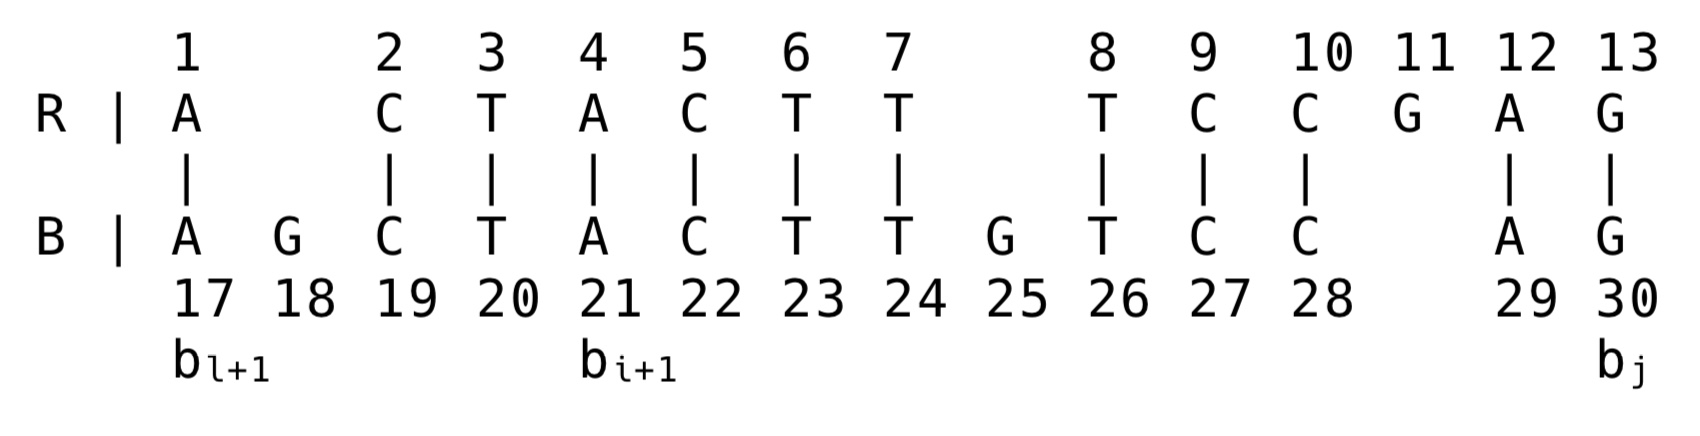
\includegraphics[width=120mm]{InfixExample.jpeg}
\caption{Poklapanje između uzokra $R = ACTACTTTCCGAG$ i podniza teksta $B = b_{17}\dots b_{30} = \dots AGCTACTTGTCCAG \dots$}\label{fig:infixExample}
\end{figure}

Udaljenost između ta dva niza je $k=3$. Iz toga slijedi da je udaljenost nekog podniza uzorka $R$ i podniza teksta $b_{i+1}\dots b_{j}$ sigurno $\leq k$. U prethodnom primjeru, za podniz uzorka $r_{4}\dots r_{13}$, postoji barem $30-20-3$ ($j-i-k$) znakova koji se poklapaju s podnizom teksta $b_{21}\dots b_{30}$. Podniz uzorka možemo podijeliti na najviše $k+1$ uzastopnih podnizova, takvih da se svaki od tih podnizova u potpunosti poklapa s podnizom teksta, odnosno podniz dobivamo ako niz podijelimo na mjestima gdje se uzorak i tekst razlikuju. Uvedimo sada trojku $(p,c,f)$, gdje $p$ označava poziciju u tekstu, $c$ označava poziciju u uzorku te $f$ označava duljinu poklapanja. Ako se podniz teksta $b_{p+1}\dots b_{p+f}$ poklapa s podnizom uzorka $r_{c+1}\dots r_{c+f}$, te ako je $r_{c+f+1}\neq b_{p+f+1}$, tada ćemo to poklapanje zapisati prethodno definiranom trojkom $(p,c,f)$ (u primjeru, jedna od trojki je $(18,1,6)$). Isto tako, znakove podniza teksta $b_{i+1}\dots b_{j}$ za koje ne postoji poklapanje, možemo označiti trojkom $(h,0,0)$, gdje $h$ označava poziciju unutar teksta $B$, a $0$ označava da u uzorku ne postoji znak koji odgovara znaku u tekstu (u primjeru, $(17,0,0)$). Primjenom ovakve analize na podniz teksta $b_{i+1}\dots b_{j}$, podniz možemo podijeliti na $O(k)$ slijednih poklapanja i promašaja. Za podniz u primjeru to prikazujemo podnizom $(20,3,4),(24,0,0),(25,7,3),(28,11,2)$. Ovaj niz trojki označit ćemo sa $S_{20,30}$ (općenito $S_{i,j}$, gdje $i$ označava trenutnu iteraciju, a $j$ označava najdalju poziciju koju smo dosegli u tekstu).

\subsection{Detaljan opis algoritma}
Jedna iteracija algoritma bazira se na prefiksnom algoritmu opisanom u poglavlju \ref{sec:prefiksniAlg} s time da prilikom pomicanja po uzorku koristimo matricu $MAXLENGTH$ (\ref{tab:maxlength}) te niz trojki $S_{i,j}$ dobiven iz prethodne iteracije kako bi postigli ubrzanje. U jednoj iteraciji, koristit ćemo bazu prefiksnog algoritma (\ref{alg:prefix}), no uz zamjenu instrukcije [3] s novim nizom instrukcija. Umjesto da varijablu $row$ povećavamo za jedan u svakom prolazu, koristi ćemo se znanjem prethodne iteracije i matricom $MAXLENGTH$ kako bi varijablu $row$ povećali za veće iznose.

\begin{algorithm}
\caption{Algoritam za izračunavanje infiksne udaljenosti dva niza s najviše $k$ razlika}\label{alg:infix}
\begin{algorithmic}[1]
\State $\#$ $C_{CH} = C_{DE} = C_{IN} = 1$
\State $j \gets 0$
\State $S_{i,j} \gets \emptyset$
\For{$i \gets 0$ to $n-m+k$}
\For{$d \gets -(k+1)$ to $(k+1)$} 
    \State $L_{d,|d|-2} \gets -\infty$
    \If{$d<0$} \State $L_{d,|d|-1} \gets |d|-1$
    \Else \State $L_{d,|d|-1} \gets -1$
    \EndIf
\EndFor
\linebreak
\For{$e \gets 0$ to $k$}
    \For{$d \gets -e$ to $e$}
        \State $row\gets max(L_{d,e-1} + 1, L_{d-1,e-1}, L_{d+1,e-1} + 1)$
        \State Izvrši novi skup instrukcija       
        \While{$(r_{row+1} = b_{row+d+1})$}
            \State $row\gets row+1$
        \EndWhile
        \State[5] $L_{d,e}\gets row$
        \State
        \If{$(L_{d,e}=m)$}
            \State \textbf{goto} 7
        \EndIf
    \EndFor
\EndFor
	\State [7] Ako smo u trenutnoj iteraciji došli do nekih novih simbola, odnosno ako se $j$ povećao, počevši od $L_{d,k}$ (po definiciji $j=L_{d,k}+d+i$) stvorimo novi niz trojki $S_{i,j}$ na temelju analize teksta.
	\If{$(L_{d,e}=m)$}
    	\State \Return $e$
    \EndIf
    
\EndFor
\linebreak
\Return $-1$
\end{algorithmic}
\end{algorithm}

\begin{algorithm}
\caption{Nove istrukcije koje omogućuju ubrzanje infiksnog algoritma}\label{alg:infixNew}
\begin{algorithmic}[1]
        \While{$(i+row+d+1 \leq j)$}
        	\State $c \gets 0$
        	\State $f \gets 0$
            \For{$S$ in $S_{i,j}$}
            	\If{$S.p+S.f>row+d+i+1$ and $S.p=row+d+i+1$}
            		\State $c \gets S.c$
        			\State $f \gets S.f$
        			\State \textbf{break}
            	\EndIf
            \EndFor
            
            \State
            \If{$f\geq 1$}
            	\If{$f \neq MAXLENGTH[c][row]$}
            		\State $row \gets row + min(f,MAXLENGTH[c][row])$
            		\State \textbf{goto} 5
            	\Else
            		\State $row \gets row + f$
            	\EndIf
            \Else
            	\If{$r_{row+1} \neq b_{i+row+1+d}$}
            		\State \textbf{goto} 5
            	\Else
            		\State $row \gets row + 1$
            	\EndIf
            \EndIf
        \EndWhile
\end{algorithmic}
\end{algorithm}

Vratimo se sada na iteraciju $i=20$ opisanu ranije u poglavlju ($j=30$, $S_{i,j}=(20,3,4),(24,0,0),(25,7,3),(28,11,2)$). Novi skup instrukcija (Algoritam \ref{alg:infixNew}) koji zamjenjuje instrukciju [3] prefiksnog algoritma omogućava nam da, dokle god se nalazimo u djelu teksta prije $j=30$ pozicije, koristimo matricu $MAXLENGTH$ (\ref{tab:maxlength}) i niz trojki $S_{i,j}$ da varijablu $row$ povećavamo za više od 1 te tako ubrzamo algoritam. While petlja traži najduže moguće poklapanje između podnizova teksta $b_{i+row+d+1}$ i uzorka $r_{row+1}$. To postižemo uz pomoć niza $S_{i,j}$, odnosno tražimo broj $c$ u nekoj od trojki $(p,c,f)$ sadržanih u $S_{i,j}$ takav da $b_{i+row+d+1}\dots b_{i+row+d+f} = r_{c+1}\dots r_{c+f}$.

U slučaju kada u $S_{i,j}$ postoji poklapanje (postoji trojka $(p,c,f)$ takva da je $f\geq 1$), tražimo element matrice $g=MAXLENGTH[c][row]$. Tada razlikujemo dva slučaja:
\begin{enumerate}\begin{sloppypar}
\item Kada je $f\neq g$: Tada je duljina poklapanja $min(f,g)$, odnosno da je $b_{i+row+d+1}\dots b_{i+row+d+min(f,g)} = r_{row+1}\dots r_{row+min(f,g)}$ i $b_{i+row+d+min(f,g)+1} \neq r_{row+min(f,g)+1}$. To možemo zaključiti iz definicija matrice \textit{MAXLENGTH} i trojke $(p,c,f)$. Vrijednost $f\geq 1$ nam govori da smo u nekoj od prošlih iteracija algoritma već pokrili ovaj dio uzorka i teksta, te da ovdje postoji poklapanje između uzorka i teksta duljine $f$. Vrijednost $g$ nam omogućava da koristimo i vrijednosti trojke $(p,c,f)$ koje se ne odnose izravno na trenutni podniz uzorka $r_{row+1}\dots r_{row+g} $, nego se odnose na podniz $ r_{c+1}\dots r_{c+g} $ identičan trenutnom ($r_{row+1}\dots r_{row+g}=r_{c+1}\dots r_{c+g}$). Informacija o duljini $g$ podniza za koje prethodna jednakost vrijedi zapisana je u $MAXLENGTH[c][row]$.

Varijablu $row$ tada povećavamo za $min(f,g)$ i odlazimo na instrukciju [5]. U prethodnom primjeru, pretpostavimo da je $row=8$ i $d=-2$. To znači da tražimo preklapanje između $r_{9}\dots$ i $b_{27}\dots$. Trojka koja pokriva trenutni položaj je $(25,7,3)$, što znači da su znakovi na pozicijama 27 i 28 u tekstu jednaki znakovima na mjestu 9 i 10 u uzorku, odnosno $f=2$ i $c=8$ te $g=MAXLENGTH[7][7]=5$. Iz toga slijedi da se možemo pomaknuti za 2 mjesta dalje, odnosno $row = row + 2$.
\item Kada je $f = g$: Tada sigurno vrijedi da je $b_{i+row+d+1}\dots b_{i+row+d+f} = r_{row+1}\dots r_{row+f}$, no ne znamo ništa o odnosu sljedećih znakova u uzorku i tekstu, odnosno vrijedi li $b_{i+row+d+f+1} = r_{row+f+1}$. Zato, sada povećavamo $row$ za $f$ te se vraćamo na while petlju i nastavljamo algoritam.
\end{sloppypar}\end{enumerate}
Ako poklapanje koje pokriva $b_{i+row+d+1}$ ne postoji u $S_{i,j}$, tada tražimo poklapanje između $b_{i+row+d+1}$ i $r_{row+1}$. U prethodnom primjeru to bi odgovaralo stanju kada je $row=3$ i $d=1$. Ovdje opet razlikujemo dva slučaja:
\begin{enumerate}
\item Kada je $b_{i+row+d+1}\neq r_{row+1}$: Tada ne postoji poklapanje i odmah nastavljamo na instrukciju [5].
\item Kada je $b_{i+row+d+1}\neq r_{row+1}$: Tada varijablu $row$ povećavamo za 1 te se vraćamo na while petlju i nastavljamo algoritam.
\end{enumerate}

U instrukciji [7] stvaramo novi niz trojki $S_{i,j}$ ako smo došli do nekog novog znaka u tekstu. Neka $b_{\bar{j}}$ predstavlja zadnji novi znak u tekstu do kojeg smo došli u iteraciji $i$. Također, za svaku iteraciju $i$ čuvamo niz trojki za svaki $L_{d,e}$ izračunat u toj iteraciji. Za izgradnju niza trojki za $L_{d,e}$ koristit ćemo se nizom trojki njegovog prethodnika, odnosno niza trojki od ili $L_{d-1,e-1}$ ili $L_{d,e-1}$ ili $L_{d+1,e-1}$, ovisno o tome koji od njih smo odabrali na početku iteracije, na liniji 13 algoritma. Nazovimo taj niz trojki $S_{L_{d,e}}$ Uvedimo još i $l_{1}$ koji predstavlja vrijednost varijable row na početku iteracije (on je određen odabirom u liniji 13). Novi niz trojki sada gradimo tako da prvo, ako smo $l_{1}$ dobili odabirom ili $L_{d-1,e-1}$ ili $L_{d,e-1}$, dodamo trojku $(i+l_{1}+d-1,0,0)$ na kraj $S_{L_{d,e}}$. Nakon što izvršimo instrukciju [5], provjerimo je li $L_{d,e}>l_{1}$. Ako je, na kraj niza $S_{L_{d,e}}$ dodajemo trojku $(i+l_{1}+d,l_{1},L_{d,e}-l_{1})$.

Na samom kraju iteracije $i$ provjerimo za koju od $2k+1$ nizova trojki pridruženih svakom $L_{d,e}$, dolazimo najdalje u tekstu. Ako je taj index veći od $j$, odnosno ako je $L_{d,e}+d+i>j$, tada niz trojki $S_{i,j}$ postavljamo na $S_{L_{d,e}}$.

\subsection{Vremenska složenost infiksnog algoritma}\label{ssec:slozenostInfix}
U najgorem slučaju, vremenska složenost stare instrukcije [3] (instrukcija gdje se varijabla $row$ može povećati samo za 1) prefiksnog algoritma bila je $O(kn)$. Za izračun složenosti novog skupa instrukcija, koristit ćemo se činjenicom da u svakom trenutku održavamo najviše $2k+1$ dijagonalu te da niz $S_{i,j}$ sadrži najviše $2k+1$ trojki. Za bilo koju operaciju na dijagonali možemo pretpostaviti da se radi ili o pronalasku razlike (takvih operacija ima najviše $k$) ili o provjeravanju trojke u nizu $S_{i,j}$. Vidimo da ovo rezultira s $O(k)$ operacija za svaku dijagonalu za svaku iteraciju $i$. Iz toga slijedi da je ukupna vremenska složenost ovog algoritma $O(k^2n)$.

\chapter{Implementacija}
Algoritam Landau-Vishkin-Nussinov implementirali smo u programskom jeziku C++, korištenjem standarda C++11. Odabrali smo jezik C++ iz više razloga, od kojih su dva glavna bila velika brzina izvođenja jezika te zato što je edlib napisan isto napisan u C++, pa smo time olakšali i ubrzali ugradnju.
\begin{sloppypar}
Programski kod implementacije zajedno s uputstvima za korištenje javno je dostupan na web starnici: \href{https://github.com/donikv/Zavrsni_Rad}{https://github.com/donikv/Zavrsni\_Rad}. Također, programski kod edliba te uputstva za korištenje dostupni su na web stranici: \href{https://github.com/Martinsos/edlib}{https://github.com/Martinsos/edlib}. Važno je napomenuti da se dalje u poglavlju detaljnije opisuje verzija implementacije algoritma koja je postojala u trenutku pisanja rada te da postoji mogućnost da se trenutne implementacije dostupne na webu razlikuje od opisane.
\end{sloppypar}
\section{Prefiksni algoritam}
U nastavku poglavlja dane su implementacije 5 osnovnih dijelova prefiksnog algoritma koje smo naveli u poglavlju \ref{sec:prefiksniAlg}. Definirajmo razred $EqualityDefinition$ koji nam omogućava da proširimo relaciju jednakosti nad znakovima abecede od kojih su uzorak i tekst načinjeni. Kako bi mogli koristiti taj razred, prije početka algoritma, uzorak i tekst transformiramo u format koji nam omogućava brzo pronalaženje proširene relacije jednakosti pomoću razreda $EqualityDefinition$ te prilikom te transformacije također formiramo i abecedu s kojom su nizovi napravljeni. Definicija razreda $EqualityDefinition$ preuzeta je iz alata edlib. Inicijalizacija tog razeda bazira se na izgradnji matrice gdje nam element na poziciji $a,b$ govori jesu li znakovi koji se transformiraju u $a$ i $b$ jednaki. Transformacija znakova je jednostavna pretvorba znaka u njegovu poziciju u nizu koji predstavlja abecedu. To nam omogućava da provjera jednakosti ima složenost $O(1)$. 

 
\subsection{Inicijalizacija vrijednosti}
U sljedećem odsječku koda prikazana je inicijalizacija vrijednosti na početku algoritma. Vrijednosti koje se inicijaliziraju su vrijednosti koje se nalaze izvan matrice (\ref{tab:matricaAlg2}) te su njihove vrijednosti izabrane na takav način da se nikada ne može dogoditi da se u koraku [2] algoritma neka od tih vrijednosti odabere kao maksimalna. Vrijednost $-5$ dana je kao zamjena za $-\infty$, jer je to dovoljno velika negativna vrijednost da će sigurno uvijek biti manja od svih $L_{d,e}$. Također važno je primijetiti da mapa $cigarDict$ sadrži kopije vektora znakova, a razlog za to je jer se vektor $cv$ konstantno nadograđuje na vektore svojih prethodnika kako napredujemo kroz algoritam, no njegovu vrijednost u svakom koraku (za svaki izračunati $L_{d,e}$) moramo pospremiti kako bi kasnije mogli odabrati optimalni put. Vrijednost varijable $nk$ nam omogućava da s donje strane ograničimo udaljenost, odnosno definiramo najmanju moguću udaljenost između nizova. Razredi $Hasher$ i $EqualFn$ su pomoćni razredi koji omogućavaju pohranu strukture $L$ u hash tablicu.
\newline
\begin{lstlisting}
unordered_map<L,vector<char>, Hasher, EqualFn> cigarDict;
vector<char> cv;

for (int d = -(k); d<=k; d++){
	if(d>=-nk && d<=nk && d!=0) continue;
    D[L{d,abs(d)-2}] = -5;
    if(d<0) D[L{d, -d-1}] = -d-1;
    else D[L{d, d-1}] = -1;

    if(cigar){
        cigarDict[L{d,abs(d)-2}] = cv;
        cigarDict[L{d,abs(d)-1}] = cv;
    }
}
\end{lstlisting}


\subsection{Odabir vrijednosti varijable $row$}
Način odabira nove vrijednosti varijable $row$ detaljno je opisan u poglavlju \ref{sec:prefiksniAlg}. Funkcija max prima vrijednost $num$, u koju pohranjuje vrijednost koja je od predanih $L_{d,e}$ vrijednosti bila odabrana. Ta informacija nam je potrebna u drugom dijelu odsječka kako bi mogli odrediti na koju od vrijednost moramo dodati na kraj vektora $cv$. Također, isto kao i u prošlom odsječku, vrijednost $-5$ predstavlja zamjenu za vrijednost $-\infty$.
\newline
\begin{lstlisting}
if(d==-e){
    row = max(D[L{d,e-1}]+1, D[L{d+1,e-1}]+1, -5, &num);
} else if (d==e) {
    row = max(D[L{d,e-1}]+1, -5, D[L{d-1,e-1}], &num);
} else {
    row = max(D[L{d,e-1}]+1, D[L{d+1,e-1}]+1, D[L{d-1,e-1}], &num);
}


if(cigar){
    switch (num){
        case 1:
            cv = cigarDict[L{d,e-1}];
            if(e!=0)
                cv.push_back('I');
            break;
        case 2:
            cv = cigarDict[L{d+1,e-1}];
            cv.push_back('X');
            break;
        case 3:
            cv = cigarDict[L{d-1,e-1}];
            cv.push_back('D');
            break;
    }
}
\end{lstlisting}

\subsection{Napredovanje po dijagonali}\label{ssec:diagonal}
Nakon odabira trenutne vrijednosti varijable $row$, dolazimo do glavnog dijela algoritma, odnosno djela gdje iteriramo po dijagonali $d$ sve dok su vrijednosti uzorka $R$ na mjestu $row$ jednake vrijednostima teksta na $B$ na mjestu $row+d+bStart$. Varijabla $bStart$ omogućava nam da na početku algoritma zadamo poziciju unutar teksta $B$ od koje ćemo početi tražiti udaljenost. Na kraju odsječka obavljamo pridruživanje trenutne vrijednosti varijable $row$ trenutno aktivnom $L_{d,e}$. Varijabla $equality$ je primjerak razreda $EqualityDefinition$.
\newline
\begin{lstlisting}
while(equality.areEqual(R[row], B[row+d+bStart]) && row<m) {
    if (cigar) cv.push_back('=');
    row++;
}
D[L{d,e}] = row;
if (cigar) cigarDict[L{d,e}] = cv;
\end{lstlisting}

\subsection{Kraj algoritma}
Prefiksni algoritam završava ako u nekom trenutku vrijednost varijable $row$ dosegne vrijednost $m$ koja predstavlja duljinu uzorka $R$ ili ako isprobamo svaku od $2k+1$ dijagonalu i ni u jednom slučaju ne dođemo do kraja uzroka.
\newline
\begin{lstlisting}
for (int e = nk; e<=k; e++) {
    for(int d = -e; d<=e; d++) {

        //Tijelo algoritma, koje je opisano ranije u poglavlju

        if(row == m) {
            if (cigar) cigarVector = cv;
        }
    }
}
return -1;
\end{lstlisting}

\section{Infiksni algoritam}
Implementacija infiksnog algoritma bazira se na ponavljanju prefiksnog algoritma $n-m+k+1$ puta, uz optimizaciju napredovanja po dijagonali prikazanog u potpoglavlju \ref{ssec:diagonal}. Infiksni algoritam detaljno je opisan u poglavlju \ref{sec:infiksniAlg}.
 
\subsection{Optimizirano napredovanje po dijagonali}
Ubrzanje napredovanja po dijagonali postižemo korištenjem znanja iz prošlih iteracija kako bi mogli varijablu $row$ povećavati za iznose veće od 1. Ovdje se koristimo nizom trojki $(p,c,f)$ $S_{i,j}$. U ispod prikazanom odsječku je while petlja koja nam omogućava da dokle god se nalazimo u već istraženom dijelu teksta ($row+d+i\leq j$) koristimo $S_{i,j}$ da napredujemo brže. Ovaj dio algoritma opisan je pseudokodom te popratnim objašnjenjem u poglavlju \ref{sec:infiksniAlg} (Algoritam \ref{alg:infixNew}). 
\newline
\begin{lstlisting}
l1 = row;
while(row+d+i<=j){
    unsigned int c=0;
    unsigned int f=0;
    for(const auto& t: Sij){
        if(t.p+t.f>row+d+i && t.p==row+d+i){
            f=t.f;
            c=t.c;
            break;
        }
    }

    if(f>=1) {
        if(f != MAXLENGTH[c*m+row]) {
            row += std::min(f,MAXLENGTH[c*m+row]);
            if (cigar) {
                for(int a=0;a<std::min(f,MAXLENGTH[c*m+row]);a++) cv.push_back('=');
            }
            goto inst5;
        } else {
            if (cigar) {
                for(int a=0;a<f;a++) cv.push_back('=');
            }
            row += f;
        }
    } else {
        if(!(equality.areEqual(R[row], B[row+d+i]))){
            goto inst5;
        } else {
            if (cigar) cv.push_back('=');
            row++;
        }
    }
}
\end{lstlisting}

\subsection{Stvaranje novog niza trojki za trenutni $L_{d,e}$}
Svaki puta kada izračunamo novi $L_{d,e}$ potrebno je izračunati i pripadni niz trojki $S_{i,j}$ koji opisuju kako smo došli do pozicije unutar uzorka koja je u njemu zapisana. Varijabla $pickedL$ sadrži informaciju o tome koji $L_{\bar{d},e-1}$ (gdje $\bar{d}$ može biti ista dijagonala ili dijagonala ispod ili iznad trenutne dijagonale $d$) smo izabrali kao prethodnik prilikom izračunavanja trenutnog $L_{d,e}$. Novi niz trojki $S$ za trenutni $L$ izgradit ćemo na temelju niza $S$ za prethodni $L$. Ako se prethodni $L$ nalazio na dijagonali ispod ili na istoj dijagonali tada ćemo u niz $S$ na kraj dodati trojku $(i+l_1+d-1,0,0)$. Zatim, ako smo varijablu $row$ povećali za barem 1 (varijabla $l_1$ čuva vrijednost varijable $row$ s početka iteracije), dodajemo na kraj niza $S$ trojku $(i+l_1+d, l_1, row-l_1)$. Ovaj postupak detaljno je opisan i objašnjen kroz primjer u poglavlju \ref{primjer}.
\newline
\begin{lstlisting}
inst5:
D[L{d,e}] = row;
if (cigar) cigarDict[L{d,e}] = cv;

L pickedL; //get L that was picked as the L that gives the maximum row
if(num==1) { pickedL.d = d; pickedL.e = e-1; }
else if(num == 2){ pickedL.d = d+1; pickedL.e = e-1; }
else { pickedL.d = d-1; pickedL.e = e-1; }

std::vector<Triple> sequenceForCurrentL = lSeqMap[pickedL];

if((pickedL.d == d-1 || pickedL.d == d) && l1+d>0) sequenceForCurrentL.push_back(Triple{i+l1+d-1,0,0});
if(row>l1) sequenceForCurrentL.push_back(Triple{i+l1+d, l1, row-l1});
lSeqMap[L{d,e}] = sequenceForCurrentL;

if(row == m){
    goto inst7;
}
\end{lstlisting}


\subsection{Obabir novog niza $S_{i,j}$}
U ovom dijelu algoritma provjeravamo jesmo li se pomaknuli dalje u tekstu nego prije. U slučaju kada je $row+d+i\leq j$ tada to nije slučaj te preskačemo ovaj cijeli dio algoritma. U suprotnom, tražimo prvo pojavljivanje niza $S_{i,j}$ za koje je zadnja pozicija zapisana u trojki $(p,c,f)$ veća ili jednaka trenutnom $j$. Taj niz odabiremo kao novi $S_{i,j}$ te prelazimo u sljedeću iteraciju u slučaju da nismo došli do kraja uzorka. Inače vratimo trenutnu vrijednost $e$, odnosno udaljenost nizova.
\newline
\begin{lstlisting}
inst7:
if(i+row+d<=j) continue;
j = i+row+d;

L current_L;

for(int l = -k; l<=k; l++){
    current_L = L{l,k};
    std::vector<Triple> sequenceForCurrentL = lSeqMap[current_L];
    if(sequenceForCurrentL.size()<=0) continue;

    if((sequenceForCurrentL.back().p+sequenceForCurrentL.back().f)>=j) {
        Sij = sequenceForCurrentL;
        break;
    }
}
if(row == m) { 
    if (cigar) cigarVector = cigarDict[current_L]; 
    return e; 
}
\end{lstlisting}

\section{Ugradnja u edlib}
U nastavku dan je odsječak koda koji prikazuje najjednostavniju predloženu metodu ugradnje prefiksne implementacije algoritma Landau-Vishkin-Nussinov u edlibovu glavnu metodu za traženje poravnanja. Edlib koristi drugačije nazivlje, tako da varijabla $query$ predstavlja uzorak, a $target$ predstavlja tekst. Alat i biblioteka edlib detaljnije je opisan u radu \cite{edlib}. Prijedlog za ugradnju prefiksnog algoritma u edlib dostupan je kao \textit{Pull Request} na web stranici: \href{https://github.com/Martinsos/edlib/pull/119}{https://github.com/Martinsos/edlib/pull/119}.%TODO otvoritit pull request i kopirati link 
\newline
\begin{lstlisting}
bool useLV = queryLength < 500 && config.mode == EDLIB_MODE_SHW;
if (useLV) {
    vector<unsigned char> R(query, query + queryLength); vector<unsigned char> B(target, target + targetLength); vector<unsigned char> cigarVector;
    
    int k = config.k < 0 ? queryLength : config.k;
    result.endLocations = (int *) malloc(sizeof(int) * 1);
    result.editDistance = landauVishkinAlignPrefix(R, B, k, equalityDefinition, config.task == EDLIB_TASK_PATH, cigarVector, result.endLocations);

    if(result.editDistance>=0) {
        if(config.task == EDLIB_TASK_PATH) {
            result.alignmentLength = cigarVector.size();
            unsigned char* alignment = new unsigned char[result.alignmentLength];
            for(int i=0;i<result.alignmentLength;i++) alignment[i] = cigarVector[i];
            result.alignment = alignment;
        }

        result.startLocations = (int *) malloc(sizeof(int) * 1);
        result.startLocations[0] = 0;
        result.numLocations = 1;
    }
    return result;
}
\end{lstlisting}

\chapter{Rezultati}\label{chapter:results}
Algoritam Landau-Vishkin-Nussinov dijeli se na dva algoritma, jedan za određivanje prefiksne udaljenosti nizova, a drugi za određivanje infiksne udaljenosti nizova, dokle god je ta udaljenost manja od $k$. Uvođenjem tog ograničenja na rezultat, vremenska složenost prefiksnog algoritma postaje $O(km)$, a infiksnog algoritma $O(k^2n)$, gdje je $m$ duljina uzorka, a $n$ duljina teksta. Iz toga možemo zaključiti da će ovakav algoritam imati najveće ubrzanje za kratke nizove, s relativno malim brojem razlika između njih.

\section{Usporedba s edlibom}
Brzina implementacije opisane u ovom radu testirana je u ovisnosti o alatu edlib. Testiranje je provedeno s jednim tekstom i nizom različitih uzoraka. Niz koji je korišten kao tekst bio je zapis genoma bakterije \textit{Escherichie coli}. Duljina teksta $n$ iznosila je oko 5 milijuna proteinskih baza, dok su duljine korištenih uzoraka varirale su od 50 do 500 proteinskih baza. Nizovi su bili zapisani u FASTA formatu (\cite{FASTA}) te je za njihovo učitavanje korišten jednostavni parser koji u linearnom vremenu učitava niz u memoriju. Vrijeme potrebno za učitavanje nizova također je ulazilo u vrijeme koje je testirano. U tablicama \ref{tab:resultsPrefix50}, \ref{tab:resultsPrefix100}, \ref{tab:resultsPrefix250} i \ref{tab:resultsPrefix500} prikazani su rezultati testiranja naše implementacije i edliba. Prvi stupac tablice određuje uzorak na kojem je testiranje provedeno, a drugi stupac prikazuje duljinu uzorka. U trećem stupcu nalazi se vrsta algoritma koji je korišten, gdje Edlib označava obično traženje udaljenosti, Edlib (path) označava traženje poravnanja i optimalnog puta, dok LandauVishkin označava korištenje naše implementacije. Sljedeći stupac prikazuje prosječno vrijeme trajanja algoritma u sekundama za 100 ponavljanja, dok se u zadnjem stupcu nalazi prefiksna udaljenost uzorka i teksta. Vidljivo je da je naša implementacija na nekim, a pogotovo na vrlo kratkim primjerima brža i za više od 100 puta od edliba. Takvi rezultati su očekivani s obzirom na to da je algoritam Landau-Vishkin-Nussinov pogodan za kratke, slične nizove, dok edlib najveće ubrzanje dobiva kod dugačkih, sličnih nizova. Usporedba edliba s drugim algoritmima dana je u radu \cite{edlib}.

\begin{table}[]
\centering
\begin{tabular}{|l|l|l|l|l|}
\hline
\multicolumn{1}{|c|}{Uzorak} & \multicolumn{1}{c|}{m} & \multicolumn{1}{c|}{Algoritam} & \multicolumn{1}{c|}{Vrijeme} & \multicolumn{1}{c|}{Udaljenost} \\ \hline
50bp/mutated\_60\_perc.fasta & 50                     & Edlib                          & 0.4526                       & 22                              \\ \hline
50bp/mutated\_60\_perc.fasta & 50                     & Edlib (path)                   & 0.4529                       & 22                              \\ \hline
50bp/mutated\_60\_perc.fasta & 50                     & LandauVishkin                  & 0.0158                       & 22                              \\ \hline
50bp/mutated\_70\_perc.fasta & 50                     & Edlib                          & 0.4511                       & 15                              \\ \hline
50bp/mutated\_70\_perc.fasta & 50                     & Edlib (path)                   & 0.4585                       & 15                              \\ \hline
50bp/mutated\_70\_perc.fasta & 50                     & LandauVishkin                  & 0.0097                       & 15                              \\ \hline
50bp/mutated\_80\_perc.fasta & 50                     & Edlib                          & 0.4552                       & 11                              \\ \hline
50bp/mutated\_80\_perc.fasta & 50                     & Edlib (path)                   & 0.4506                       & 11                              \\ \hline
50bp/mutated\_80\_perc.fasta & 50                     & LandauVishkin                  & 0.0060                       & 11                              \\ \hline
50bp/mutated\_90\_perc.fasta & 50                     & Edlib                          & 0.4501                       & 4                               \\ \hline
50bp/mutated\_90\_perc.fasta & 50                     & Edlib (path)                   & 0.4520                       & 4                               \\ \hline
50bp/mutated\_90\_perc.fasta & 50                     & LandauVishkin                  & 0.0028                       & 4                               \\ \hline
50bp/mutated\_94\_perc.fasta & 50                     & Edlib                          & 0.4527                       & 3                               \\ \hline
50bp/mutated\_94\_perc.fasta & 50                     & Edlib (path)                   & 0.4529                       & 3                               \\ \hline
50bp/mutated\_94\_perc.fasta & 50                     & LandauVishkin                  & 0.0026                       & 3                               \\ \hline
50bp/mutated\_97\_perc.fasta & 50                     & Edlib                          & 0.4508                       & 3                               \\ \hline
50bp/mutated\_97\_perc.fasta & 50                     & Edlib (path)                   & 0.4523                       & 3                               \\ \hline
50bp/mutated\_97\_perc.fasta & 50                     & LandauVishkin                  & 0.0027                       & 3                               \\ \hline
50bp/mutated\_99\_perc.fasta & 50                     & Edlib                          & 0.4505                       & 1                               \\ \hline
50bp/mutated\_99\_perc.fasta & 50                     & Edlib (path)                   & 0.4540                       & 1                               \\ \hline
50bp/mutated\_99\_perc.fasta & 50                     & LandauVishkin                  & 0.0024                       & 1                               \\ \hline
\end{tabular}
\caption{Tablica koja prikazuje rezultate testiranja implementacije prefiksnog algoritma Landau-Vishkin-Nussinov i alata edlib na uzorcima duljine 50 proteinskih baza.}
\label{tab:resultsPrefix50}
\end{table}

\begin{table}[]
\centering
\begin{tabular}{|l|l|l|l|l|}
\hline
\multicolumn{1}{|c|}{Uzorak} & \multicolumn{1}{c|}{m} & \multicolumn{1}{c|}{Algoritam} & \multicolumn{1}{c|}{Vrijeme} & \multicolumn{1}{c|}{Udaljenost} \\ \hline
100bp/mutated\_60\_perc.fasta & 100 & Edlib & 0.4523 & 47 \\ \hline
100bp/mutated\_60\_perc.fasta & 100 & Edlib (path) & 0.4637 & 47 \\ \hline
100bp/mutated\_60\_perc.fasta & 100 & LandauVishkin & 0.0649 & 47 \\ \hline
100bp/mutated\_70\_perc.fasta & 100 & Edlib & 0.4543 & 35 \\ \hline
100bp/mutated\_70\_perc.fasta & 100 & Edlib (path) & 0.4565 & 35 \\ \hline
100bp/mutated\_70\_perc.fasta & 100 & LandauVishkin & 0.0376 & 35 \\ \hline
100bp/mutated\_80\_perc.fasta & 100 & Edlib & 0.4520 & 22 \\ \hline
100bp/mutated\_80\_perc.fasta & 100 & Edlib (path) & 0.4626 & 22 \\ \hline
100bp/mutated\_80\_perc.fasta & 100 & LandauVishkin & 0.0197 & 22 \\ \hline
100bp/mutated\_90\_perc.fasta & 100 & Edlib & 0.4520 & 9 \\ \hline
100bp/mutated\_90\_perc.fasta & 100 & Edlib (path) & 0.4540 & 9 \\ \hline
100bp/mutated\_90\_perc.fasta & 100 & LandauVishkin & 0.0075 & 9 \\ \hline
100bp/mutated\_94\_perc.fasta & 100 & Edlib & 0.4531 & 7 \\ \hline
100bp/mutated\_94\_perc.fasta & 100 & Edlib (path) & 0.4546 & 7 \\ \hline
100bp/mutated\_94\_perc.fasta & 100 & LandauVishkin & 0.0071 & 7 \\ \hline
100bp/mutated\_97\_perc.fasta & 100 & Edlib & 0.4541 & 4 \\ \hline
100bp/mutated\_97\_perc.fasta & 100 & Edlib (path) & 0.4538 & 4 \\ \hline
100bp/mutated\_97\_perc.fasta & 100 & LandauVishkin & 0.0058 & 4 \\ \hline
100bp/mutated\_99\_perc.fasta & 100 & Edlib & 0.4534 & 2 \\ \hline
100bp/mutated\_99\_perc.fasta & 100 & Edlib (path) & 0.4557 & 2 \\ \hline
100bp/mutated\_99\_perc.fasta & 100 & LandauVishkin & 0.0054 & 2 \\ \hline
\end{tabular}
\caption{Tablica koja prikazuje rezultate testiranja implementacije prefiksnog algoritma Landau-Vishkin-Nussinov i alata edlib na uzorcima duljine 100 proteinskih baza.}
\label{tab:resultsPrefix100}
\end{table}

\begin{table}[]
\centering
\begin{tabular}{|l|l|l|l|l|}
\hline
\multicolumn{1}{|c|}{Uzorak} & \multicolumn{1}{c|}{m} & \multicolumn{1}{c|}{Algoritam} & \multicolumn{1}{c|}{Vrijeme} & \multicolumn{1}{c|}{Udaljenost} \\ \hline
250bp/mutated\_60\_perc.fasta & 250 & Edlib & 0.4519 & 111 \\ \hline
250bp/mutated\_60\_perc.fasta & 250 & Edlib (path) & 0.4564 & 111 \\ \hline
250bp/mutated\_60\_perc.fasta & 250 & LandauVishkin & 0.3381 & 111 \\ \hline
250bp/mutated\_70\_perc.fasta & 250 & Edlib & 0.4593 & 92 \\ \hline
250bp/mutated\_70\_perc.fasta & 250 & Edlib (path) & 0.4536 & 92 \\ \hline
250bp/mutated\_70\_perc.fasta & 250 & LandauVishkin & 0.2510 & 92 \\ \hline
250bp/mutated\_80\_perc.fasta & 250 & Edlib & 0.4505 & 55 \\ \hline
250bp/mutated\_80\_perc.fasta & 250 & Edlib (path) & 0.4560 & 55 \\ \hline
250bp/mutated\_80\_perc.fasta & 250 & LandauVishkin & 0.1032 & 55 \\ \hline
250bp/mutated\_90\_perc.fasta & 250 & Edlib & 0.4520 & 32 \\ \hline
250bp/mutated\_90\_perc.fasta & 250 & Edlib (path) & 0.4543 & 32 \\ \hline
250bp/mutated\_90\_perc.fasta & 250 & LandauVishkin & 0.0456 & 32 \\ \hline
250bp/mutated\_94\_perc.fasta & 250 & Edlib & 0.4510 & 16 \\ \hline
250bp/mutated\_94\_perc.fasta & 250 & Edlib (path) & 0.4547 & 16 \\ \hline
250bp/mutated\_94\_perc.fasta & 250 & LandauVishkin & 0.0224 & 16 \\ \hline
250bp/mutated\_97\_perc.fasta & 250 & Edlib & 0.4518 & 10 \\ \hline
250bp/mutated\_97\_perc.fasta & 250 & Edlib (path) & 0.4537 & 10 \\ \hline
250bp/mutated\_97\_perc.fasta & 250 & LandauVishkin & 0.0168 & 10 \\ \hline
250bp/mutated\_99\_perc.fasta & 250 & Edlib & 0.4533 & 5 \\ \hline
250bp/mutated\_99\_perc.fasta & 250 & Edlib (path) & 0.4542 & 5 \\ \hline
250bp/mutated\_99\_perc.fasta & 250 & LandauVishkin & 0.0145 & 5 \\ \hline
\end{tabular}
\caption{Tablica koja prikazuje rezultate testiranja implementacije prefiksnog algoritma Landau-Vishkin-Nussinov i alata edlib na uzorcima duljine 250 proteinskih baza.}
\label{tab:resultsPrefix250}
\end{table}

\begin{table}[]
\centering
\begin{tabular}{|l|l|l|l|l|}
\hline
\multicolumn{1}{|c|}{Uzorak} & \multicolumn{1}{c|}{m} & \multicolumn{1}{c|}{Algoritam} & \multicolumn{1}{c|}{Vrijeme} & \multicolumn{1}{c|}{Udaljenost} \\ \hline
500bp/mutated\_60\_perc.fasta & 500 & Edlib & 0.4566 & 239 \\ \hline
500bp/mutated\_60\_perc.fasta & 500 & Edlib (path) & 0.4609 & 239 \\ \hline
\textbf{500bp/mutated\_60\_perc.fasta} & \textbf{500} & \textbf{LandauVishkin} & \textbf{3.7646} & \textbf{239} \\ \hline
500bp/mutated\_70\_perc.fasta & 500 & Edlib & 0.4558 & 180 \\ \hline
500bp/mutated\_70\_perc.fasta & 500 & Edlib (path) & 0.4606 & 180 \\ \hline
\textbf{500bp/mutated\_70\_perc.fasta} & \textbf{500} & \textbf{LandauVishkin} & \textbf{1.9114} & \textbf{180} \\ \hline
500bp/mutated\_80\_perc.fasta & 500 & Edlib & 0.4532 & 108 \\ \hline
500bp/mutated\_80\_perc.fasta & 500 & Edlib (path) & 0.4591 & 108 \\ \hline
500bp/mutated\_80\_perc.fasta & 500 & LandauVishkin & 0.3591 & 108 \\ \hline
500bp/mutated\_90\_perc.fasta & 500 & Edlib & 0.4519 & 63 \\ \hline
500bp/mutated\_90\_perc.fasta & 500 & Edlib (path) & 0.4666 & 63 \\ \hline
500bp/mutated\_90\_perc.fasta & 500 & LandauVishkin & 0.1533 & 63 \\ \hline
500bp/mutated\_94\_perc.fasta & 500 & Edlib & 0.4560 & 28 \\ \hline
500bp/mutated\_94\_perc.fasta & 500 & Edlib (path) & 0.4592 & 28 \\ \hline
500bp/mutated\_94\_perc.fasta & 500 & LandauVishkin & 0.0536 & 28 \\ \hline
500bp/mutated\_97\_perc.fasta & 500 & Edlib & 0.4611 & 15 \\ \hline
500bp/mutated\_97\_perc.fasta & 500 & Edlib (path) & 0.4798 & 15 \\ \hline
500bp/mutated\_97\_perc.fasta & 500 & LandauVishkin & 0.0349 & 15 \\ \hline
500bp/mutated\_99\_perc.fasta & 500 & Edlib & 0.4529 & 7 \\ \hline
500bp/mutated\_99\_perc.fasta & 500 & Edlib (path) & 0.4577 & 7 \\ \hline
500bp/mutated\_99\_perc.fasta & 500 & LandauVishkin & 0.0291 & 7 \\ \hline
\end{tabular}
\caption{Tablica koja prikazuje rezultate testiranja implementacije prefiksnog algoritma Landau-Vishkin-Nussinov i alata edlib na uzorcima duljine 500 proteinskih baza. Podebljano su označeni redci u kojima je algoritam Landau-Vishkin-Nussinov sporiji od edliba.}
\label{tab:resultsPrefix500}
\end{table}

\chapter{Zaključak}
Algoritam koji su 1986. godine predložili Landau, Vishkin i Nussinov \citep{Landau1986} rješava problem traženja infiksnog poravnanja između dva niza, uzorka duljine $m$ i teksta duljine $n$ ($n\geq m$), s vremenskom složenosti $O(k^2n)$, gdje $k$ predstavlja maksimalni dopušteni broj razlika između nizova. Izvod vremenske složenosti dan je u potpoglavlju \ref{ssec:slozenostInfix}. Vidimo da ovdje dobivamo najveće ubrzanje s obzirom na jednostavne algoritme ako radimo sa sličnim, kratkim nizovima. S druge strane, edlib \citep{edlib} je alat koji također rješava problem traženja poravnanja između dva niza, ali najveće ubrzanje postiže na dugim, sličnim nizovima. Zbog toga, odlučili smo se napraviti implementaciju algoritma Landau-Vishkin-Nussinov koju smo potom ugradili u edlib, kako bi omogućili brže rješavanje problema za kraće nizove. Uz infiksni algoritam, implementirali smo i prefiksnu varijaciju algoritma, jer edlib omogućava traženje prefiksnog, infiksnog i globalnog poravnanja nizova. Osim integracije u edlib, implementacija algoritma dostupna je i kao zasebna biblioteka, te ju je moguće preuzeti s web stranice: \href{https://github.com/donikv/Zavrsni_Rad}{https://github.com/donikv/Zavrsni\_Rad}.

Rezultati usporedbe implementecije algoritma Landau-Vishkin-Nussinov s edlib alatom pokazuju da je edlib u prosjeku 10 puta sporiji prilikom traženja optimalnog prefiksnog poravnanja za kratke nizove. Razlika u brzini je najveća prilikom traženja poravnanja za vrlo kratke uzorke, od oko 50 do 250 proteinskih baza, dok je za nizove od 250 do 500 bp brzina naša implementacija je skoro svaki puta brža od edliba, osim za najduže nizove s velikom udaljenosti između uzorka i teksta ($k>150$). S druge strane, edlib je brži prilikom traženja globalnog i infiksnog poravnanja, uz nepoznati $k$, dok je kod infiksnog poravnanja za poznati i mali $k$ sporiji. Detaljnija obrada rezultata dana je u poglavlju \ref{chapter:results}.

Uz to, implementacija algoritama prilagođena je tako da, uz traženje udaljenosti između nizova, omogućava i određivanje puta za koje je ta udaljenost postignuta. Da bi implementacija bila kompatibilna s edlibom, put je zapisan u formatu CIGAR, koji je opisan u poglavlju \ref{sec:cigar}.

Daljnji rad na implementaciji uključuje prilagodbu rada globalnog i infiksnog algoritma kako bi dobili bolje rezultate s obzirom na edlib. Uz to, bilo bi dobro osmisliti kvalitetnu heurističku funkciju koja bi na temelju ulaznih nizova i vrste poravnanja dobro određivala koji od algoritama treba primijeniti kako bi dobili što veće ubrzanje.

\bibliography{literatura}
\bibliographystyle{fer}

\begin{sazetak}
Vremenska i memorijska složenost optimalnog poravnanja dva niza je kvadratna što za dulje nizove rezultira jako dugačkim vremenom izvršavanja. Međutim, često imamo informaciju o tome da su nizovi slični i možemo unaprijed ograničiti kolika će biti razlika među njima. U tom slučaju koristimo algoritme koji u matrici poravnanja računaju samo glavnu dijagonalu i određen broj susjednih. Jedan od najbržih takvih algoritama opisan je u radu "An efficient string matching algorithm with k differences for nucleotide and amino acid sequences". U ovome radu predstavljena je implementacija tog algoritma, te je algoritam prilagođen kako bi se mogao ugraditi u biblioteku edlib, gdje je zadužena za traženje poravnanja između kratkih nizova.

\kljucnerijeci{bioinformatika, Landau-Viskin-Nussinov, edlib, poravnanje nizova, Levenshteinova udaljenost}
\end{sazetak}

% TODO: Navedite naslov na engleskom jeziku.
\engtitle{Landau-Vishkin-Nussinov Algorithm for Pair-wise Sequence Alignment}
\begin{abstract}
Time and memory complexity of optimal pair-wise sequence alignment is quadratic, which, for longer sequences, results in very long computation time. However, we usually have the information that the sequences are similar and we can limit the maximal edit distance between them. In that case, we use algorithms which in the alignment matrix calculate only the main diagonal and a fixed number of neighboring diagonals. One of the fastest such algorithms is described in the paper titled "An efficient string matching algorithm with k differences for nucleotide and amino acid sequences". In this paper, we present an implementation of that algorithm, and we show how the algorithm was adapted to be included into edlib library, where it is used to determine pair-wise sequence alignment of shorter sequences.

\keywords{bioinformatics, Landau-Vishkin-Nussinov, edlib, pair-wise sequence alignment, Levenshtein's distance}
\end{abstract}

\end{document}
